% =====================================================================
%  Resultados (8 diapositivas, voz C; Guia 2.4: animacion, observable contra tiempo,
%  escalar contra el parametro).
%  Las figuras salen de figuras/ (sin titulo ni caption), los parametros van al costado
%  (\params), las tablas las genera pres_format.py (tablas.tex) y los links de video salen
%  de links.json. Las cifras de la prosa se verifican contra 09-RESULTS.md.
% =====================================================================

% SLIDE res_anim | V:C | T:35
\begin{frame}{Animaciones al mismo instante}
  \begin{columns}[T]
    \begin{column}{0.325\textwidth}
      \centering
      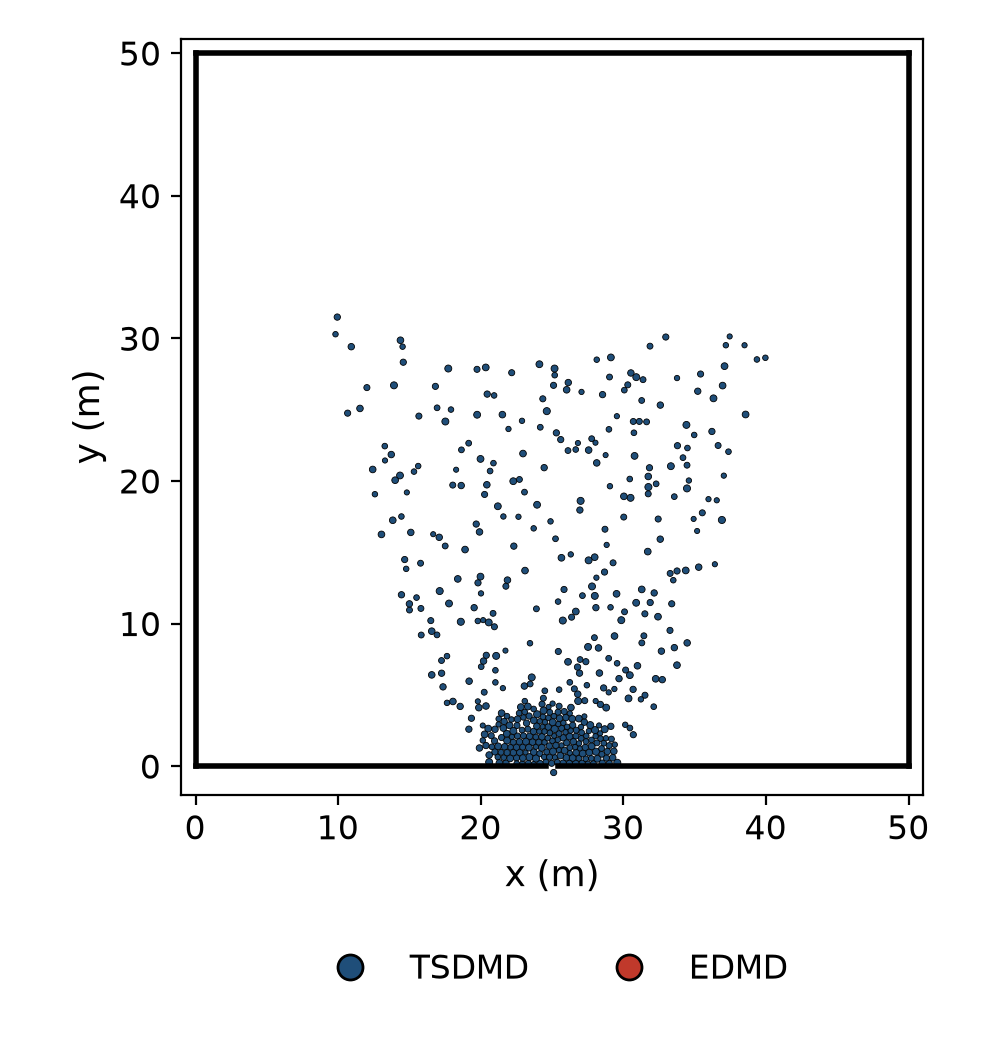
\includegraphics[width=0.74\linewidth]{frame_tsdmd.png}

      {\footnotesize\color{tsdmdc}\textbf{TSDMD}}\\
      \videolink{tsdmd_n500}
    \end{column}
    \begin{column}{0.325\textwidth}
      \centering
      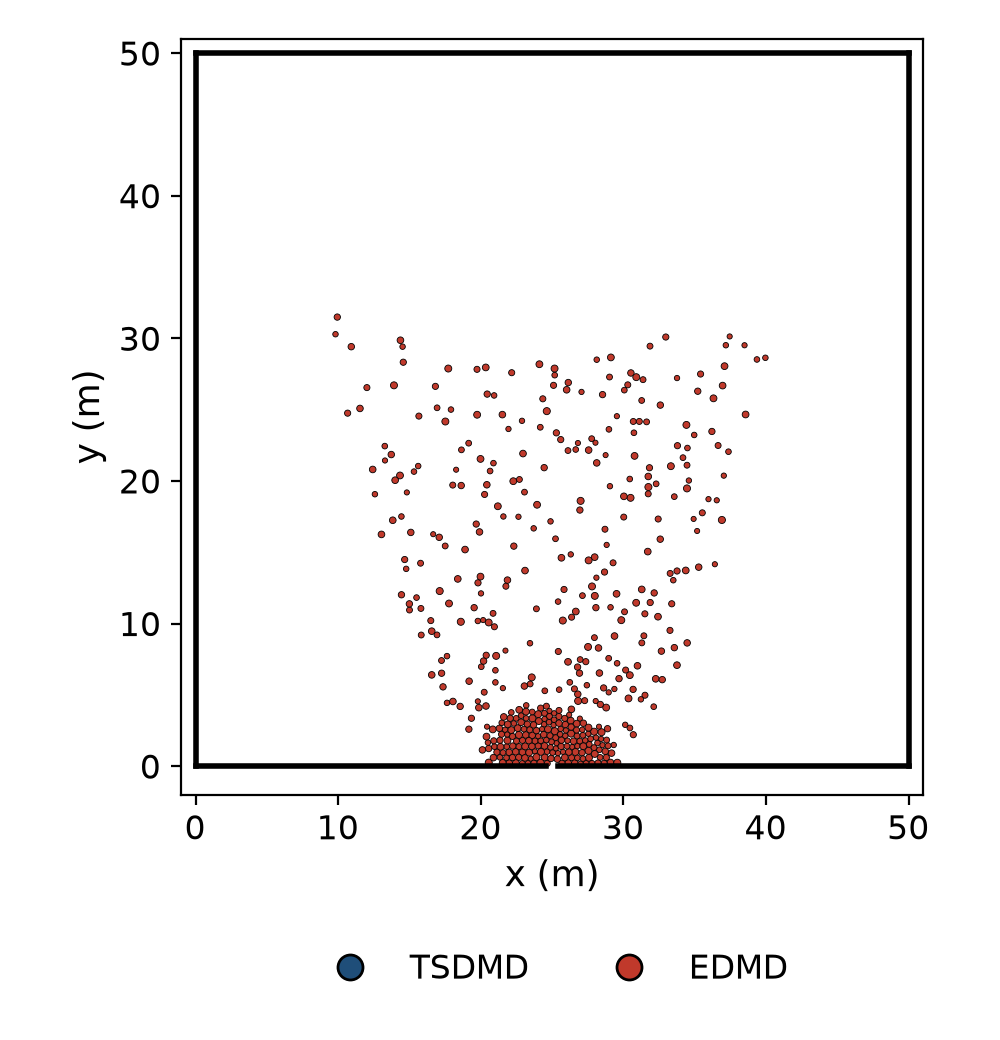
\includegraphics[width=0.74\linewidth]{frame_edmd.png}

      {\footnotesize\color{edmdc}\textbf{EDMD}}\\
      \videolink{edmd_n500}
    \end{column}
    \begin{column}{0.325\textwidth}
      \centering
      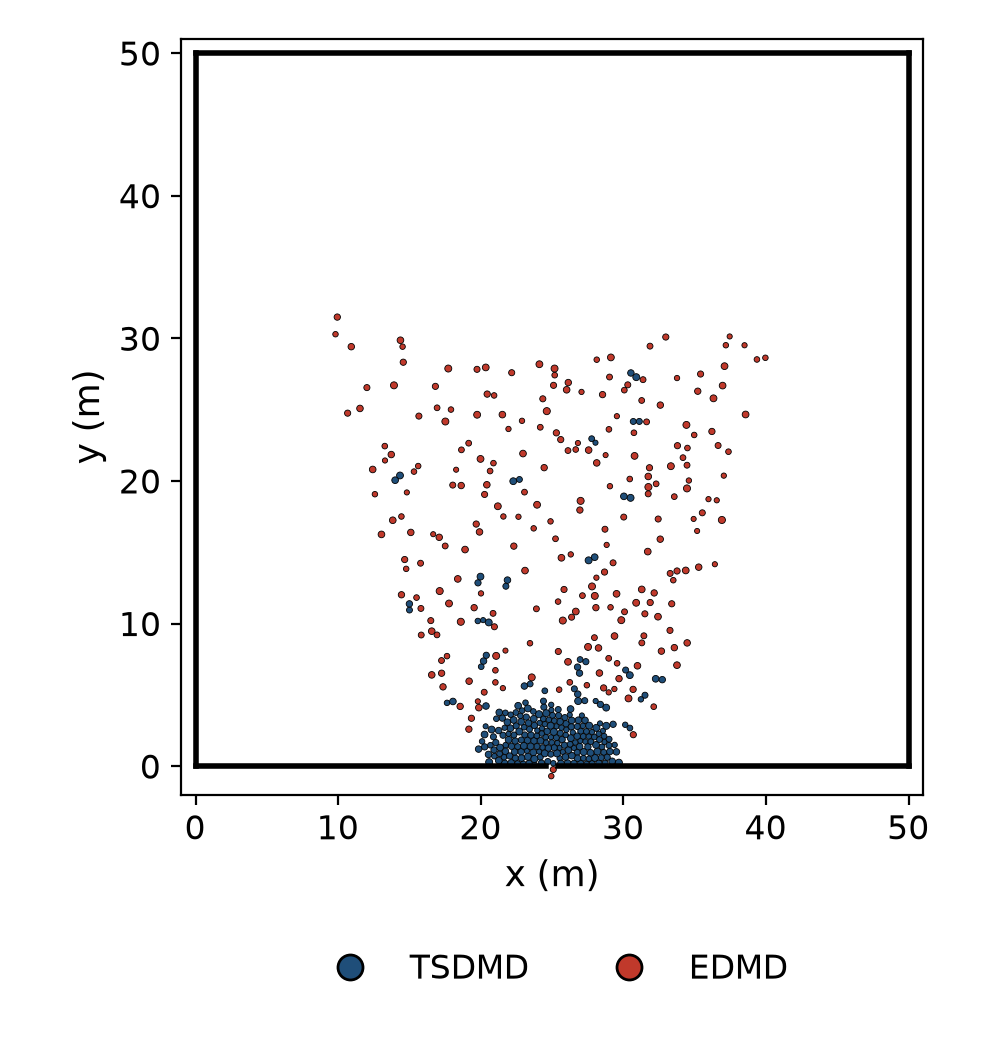
\includegraphics[width=0.74\linewidth]{frame_hybrid.png}

      {\footnotesize\color{hybc}\textbf{Híbrido}}\\
      \videolink{hybrid_n500}
    \end{column}
  \end{columns}
  \vfill
  \params{$N = 500$, $L = 50\un{m}$, semilla 18, $t = \framet\un{s}$; híbrido con $T = 0.5\un{s}$,
  $\alpha = 2$. Azul: TSDMD; rojo: EDMD (el híbrido colorea cada agente por su esquema vigente).}
\end{frame}

% SLIDE res_fraccion | V:C | T:30
\begin{frame}{Fracción de agentes por esquema en el híbrido}
  \begin{columns}[c]
    \begin{column}{0.64\textwidth}
      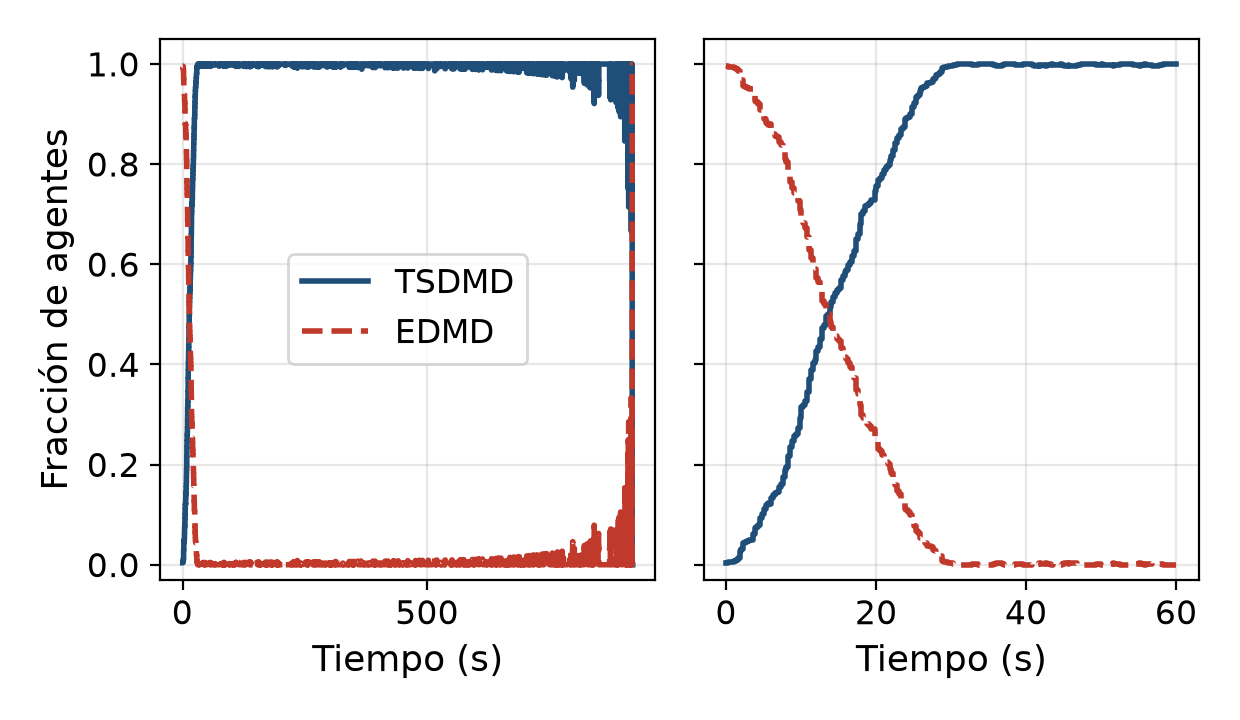
\includegraphics[width=\linewidth,height=0.84\textheight,keepaspectratio]{pres_fraction.png}
    \end{column}
    \begin{column}{0.34\textwidth}
      \params{%
        $N = 500$, $L = 50\un{m}$\\
        $T = 0.5\un{s}$, $\alpha = 2$\\
        semilla 18}

      \vspace{6pt}
      {\small Al inicio los agentes dispersos están en EDMD; hacia los $30\un{s}$ casi todos
      pasan a TSDMD (cuello de botella). Fracción TSDMD media de la corrida: $0.98$.}
    \end{column}
  \end{columns}
\end{frame}

% SLIDE res_poblacion | V:C | T:30
\begin{frame}{Población en la sala en función del tiempo}
  \begin{columns}[c]
    \begin{column}{0.64\textwidth}
      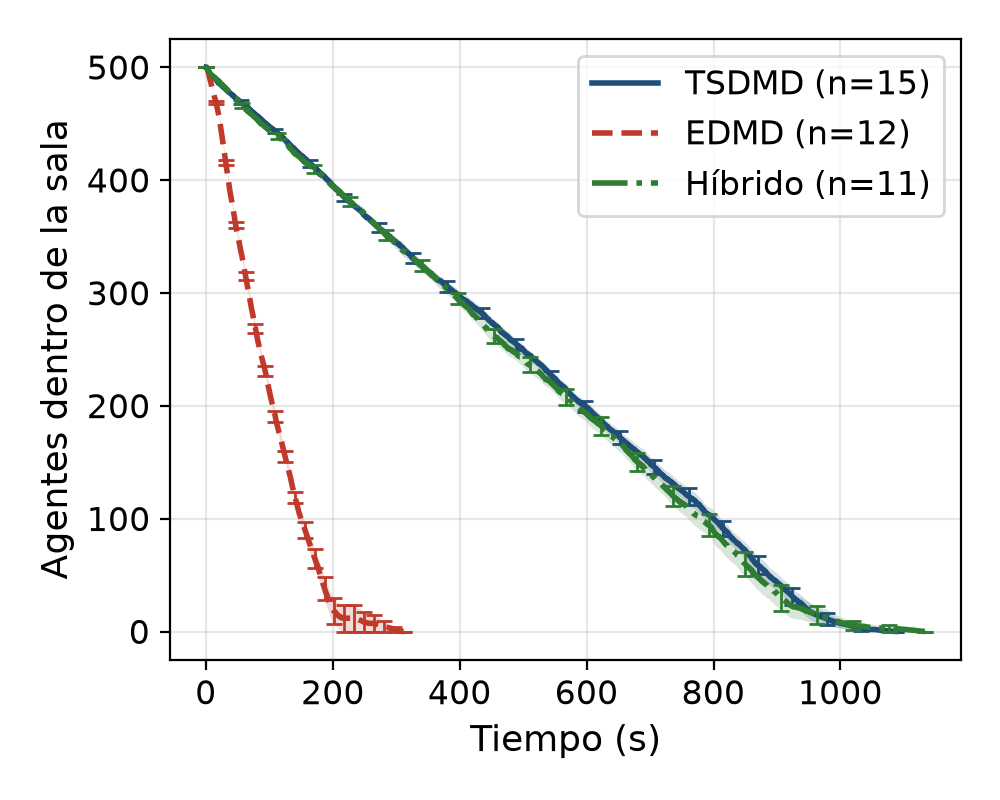
\includegraphics[width=\linewidth,height=0.84\textheight,keepaspectratio]{pres_population.png}
    \end{column}
    \begin{column}{0.34\textwidth}
      \params{%
        $N = 500$, $L = 50\un{m}$\\
        $T = 0.5\un{s}$, $\alpha = 2$\\[4pt]
        Solo corridas completas:\\
        TSDMD $n = 15$\\
        EDMD $n = 12$\\
        Híbrido $n = 11$}

      \vspace{6pt}
      {\small Las curvas del TSDMD y del híbrido casi se superponen; la del EDMD llega a $0$
      hacia los $300\un{s}$.}
    \end{column}
  \end{columns}
\end{frame}

% SLIDE res_tevac | V:C | T:40
\begin{frame}{Tiempo de evacuación según el esquema}
  \begin{columns}[c]
    \begin{column}{0.40\textwidth}
      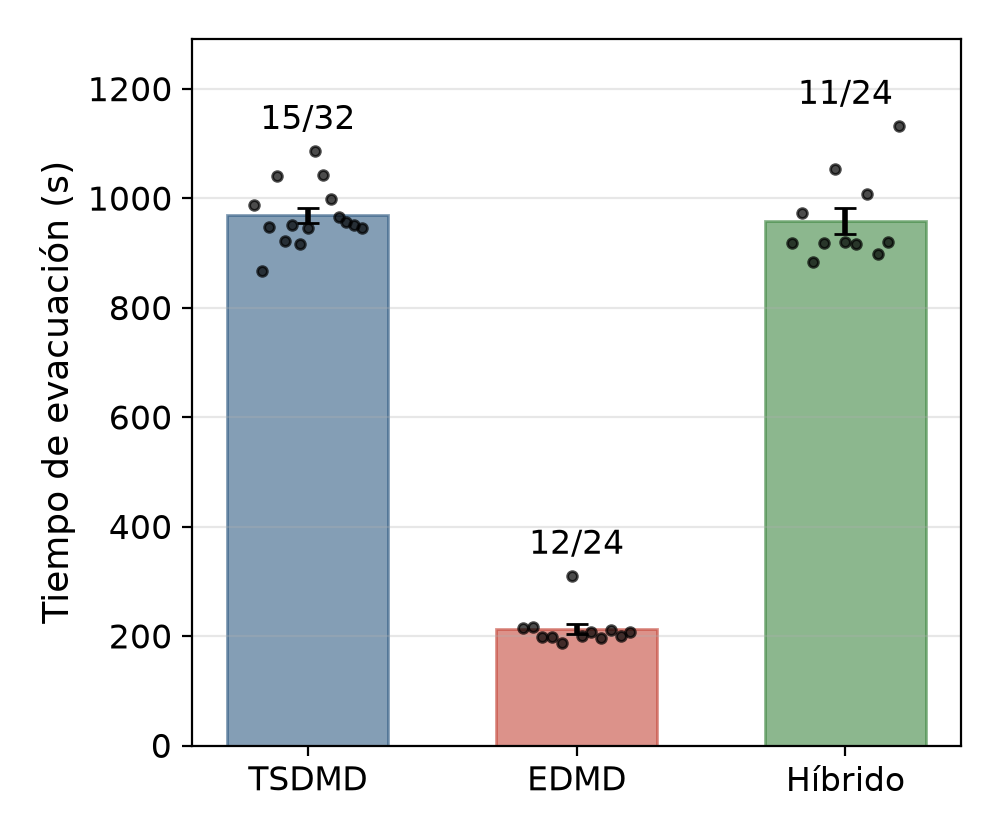
\includegraphics[width=\linewidth,height=0.84\textheight,keepaspectratio]{pres_tevac.png}
    \end{column}
    \begin{column}{0.58\textwidth}
      \resizebox{\linewidth}{!}{\tablaTevac}

      \vspace{4pt}
      \params{$N = 500$, $L = 50\un{m}$, $T = 0.5\un{s}$, $\alpha = 2$;
      $t_{max}$ 3000, 600 y $3000\un{s}$. Promedios solo sobre corridas completas.}

      \vspace{4pt}
      {\small EDMD: razón $0.22$ contra el TSDMD, $z = -44$. Híbrido: razón $0.99$ y
      $z = -0.4$, no distinguible del TSDMD con $n = 11$ y $15$.}
    \end{column}
  \end{columns}
\end{frame}

% SLIDE res_walltime | V:C | T:30
\begin{frame}{Tiempo de ejecución según el esquema}
  \begin{columns}[c]
    \begin{column}{0.40\textwidth}
      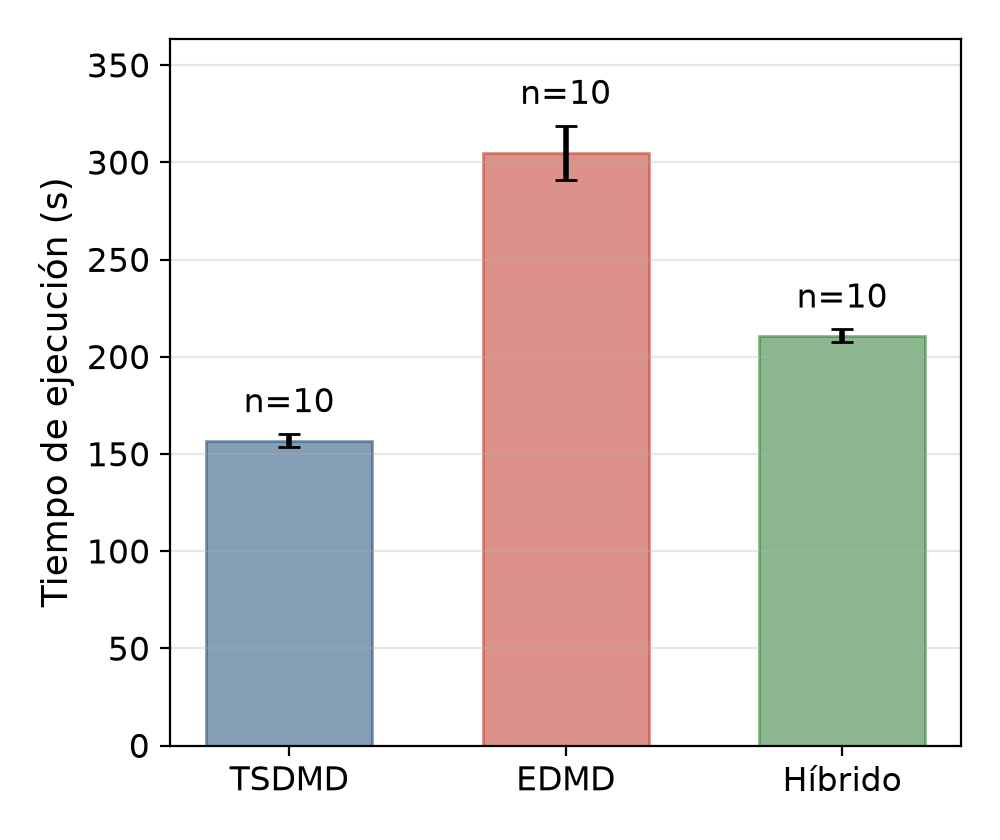
\includegraphics[width=\linewidth,height=0.84\textheight,keepaspectratio]{pres_walltime.png}
    \end{column}
    \begin{column}{0.58\textwidth}
      \resizebox{\linewidth}{!}{\tablaWall}

      \vspace{4pt}
      \params{$N = 500$, $L = 50\un{m}$, un hilo; 10 corridas completas por esquema.}

      \vspace{4pt}
      {\small Orden de costo: TSDMD, híbrido ($\times1.34$) y EDMD ($\times1.94$), inverso
      al orden de $t_{evac}$.}
    \end{column}
  \end{columns}
\end{frame}

% SLIDE res_sweep | V:C | T:40
\begin{frame}{Barrido de $T$ en el híbrido}
  \begin{columns}[c]
    \begin{column}{0.40\textwidth}
      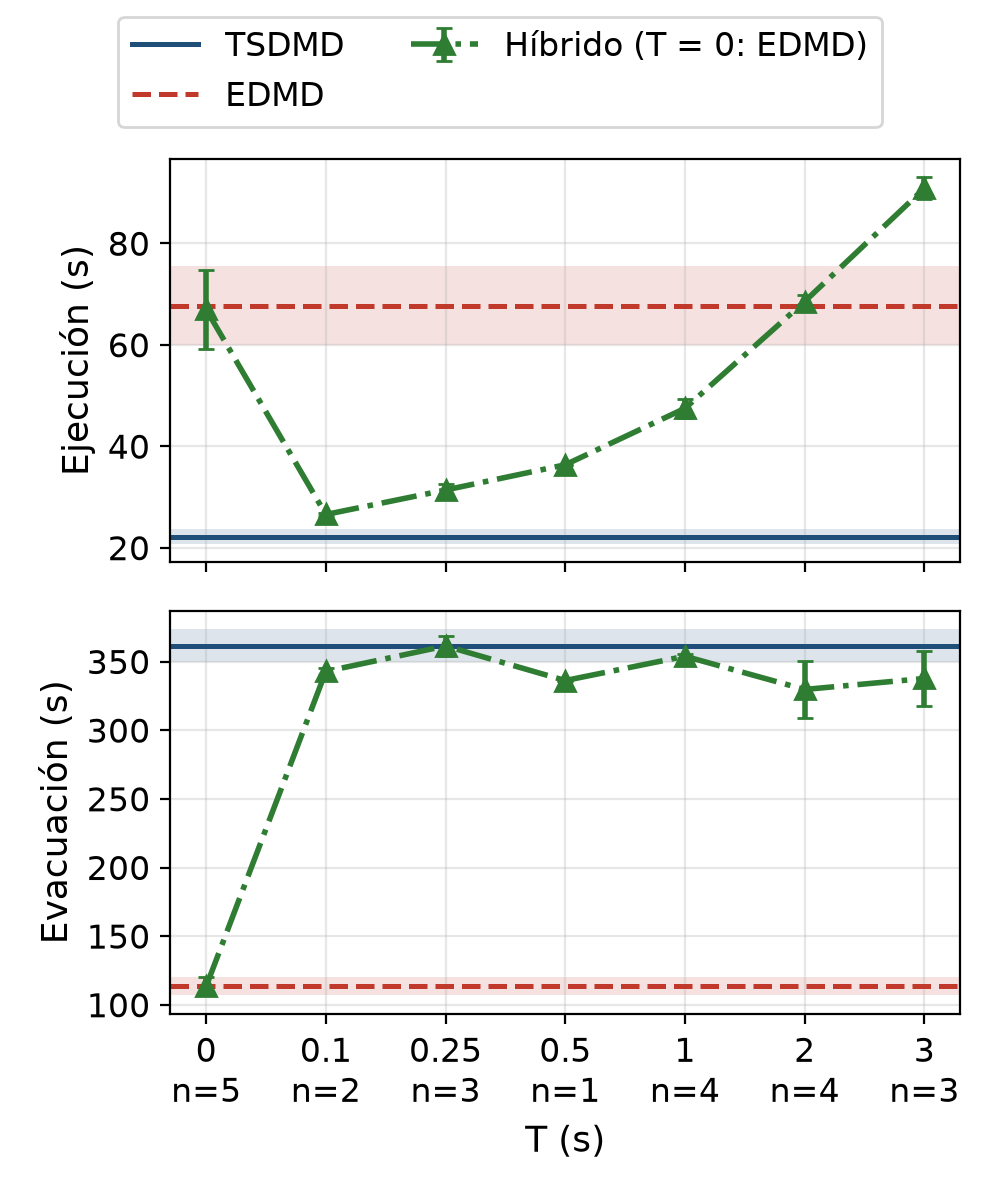
\includegraphics[width=\linewidth,height=0.84\textheight,keepaspectratio]{pres_sweep_T.png}
    \end{column}
    \begin{column}{0.58\textwidth}
      \params{$N = 200$, $L = 31.6\un{m}$, $\alpha = 2$, 5 semillas por $T$,
      $t_{max} = 600\un{s}$; $n$ completas por $T$ en el eje.}

      \vspace{6pt}
      \small
      \begin{itemize}
        \item $T = 0$ reproduce al EDMD (trayectorias idénticas).
        \item Para $T > 0$ el $t_{evac}$ queda del lado del TSDMD: ningún $T$ evaluable difiere
          en más de $2$ errores combinados; $T = 0.5\un{s}$ tiene una sola completa y no se evalúa.
        \item Tiempo de ejecución mínimo en $T = 0.1\un{s}$ ($n = 2$); crece con $T$.
      \end{itemize}
    \end{column}
  \end{columns}
\end{frame}

% SLIDE res_scale_a | V:C | T:30
\begin{frame}{Escalado en $N$: densidad inicial constante}
  \begin{columns}[c]
    \begin{column}{0.46\textwidth}
      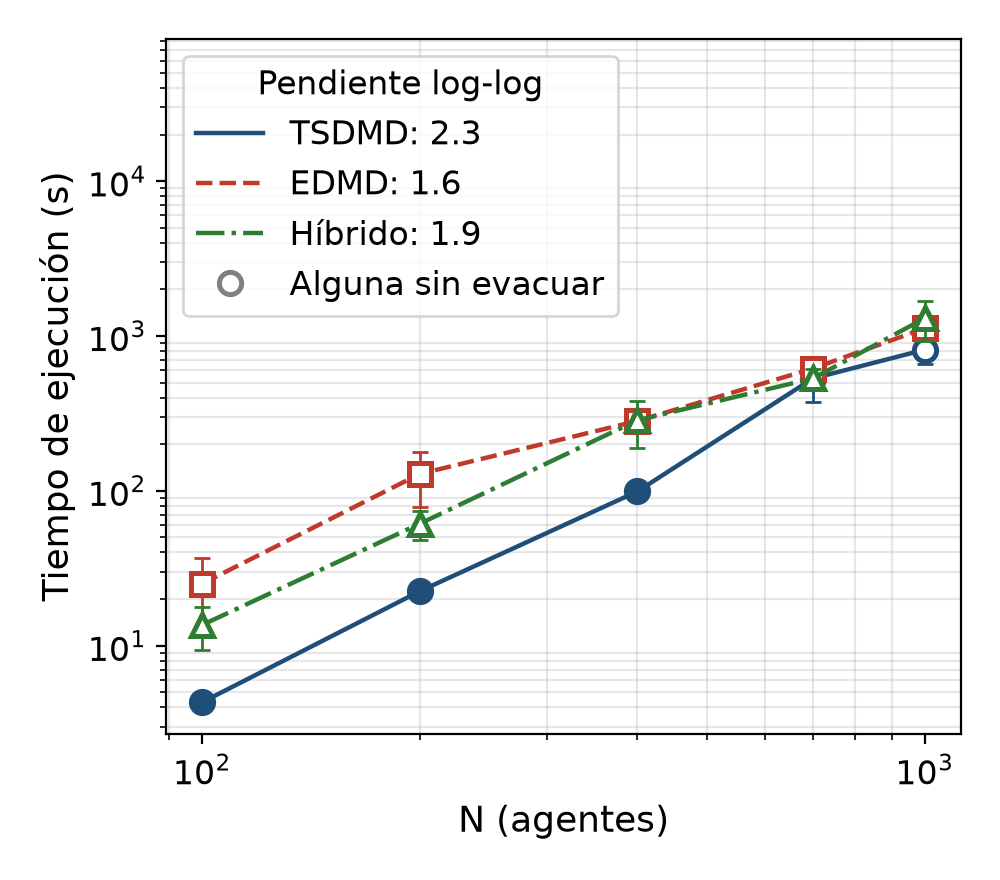
\includegraphics[width=\linewidth,height=0.84\textheight,keepaspectratio]{pres_scale_a.png}
    \end{column}
    \begin{column}{0.52\textwidth}
      \params{$N\in\{100,\,200,\,400,\,700,\,1000\}$, $L = 50\sqrt{N/500}\un{m}$,
      3 semillas por punto, $t_{max}\propto N$. Marcador hueco: alguna corrida llegó a $t_{max}$
      sin evacuar ($18$ de $45$).}

      \vspace{6pt}
      {\small Pendiente de la media observada: TSDMD $2.3$, EDMD $1.6$, híbrido $1.9$.
      \textbf{No son exponentes de costo.} Para $N\ge700$ los esquemas no se separan dentro
      del error con $3$ realizaciones por punto.}
    \end{column}
  \end{columns}
\end{frame}

% SLIDE res_scale_b | V:C | T:30
\begin{frame}{Escalado en $N$: sala fija}
  \begin{columns}[c]
    \begin{column}{0.46\textwidth}
      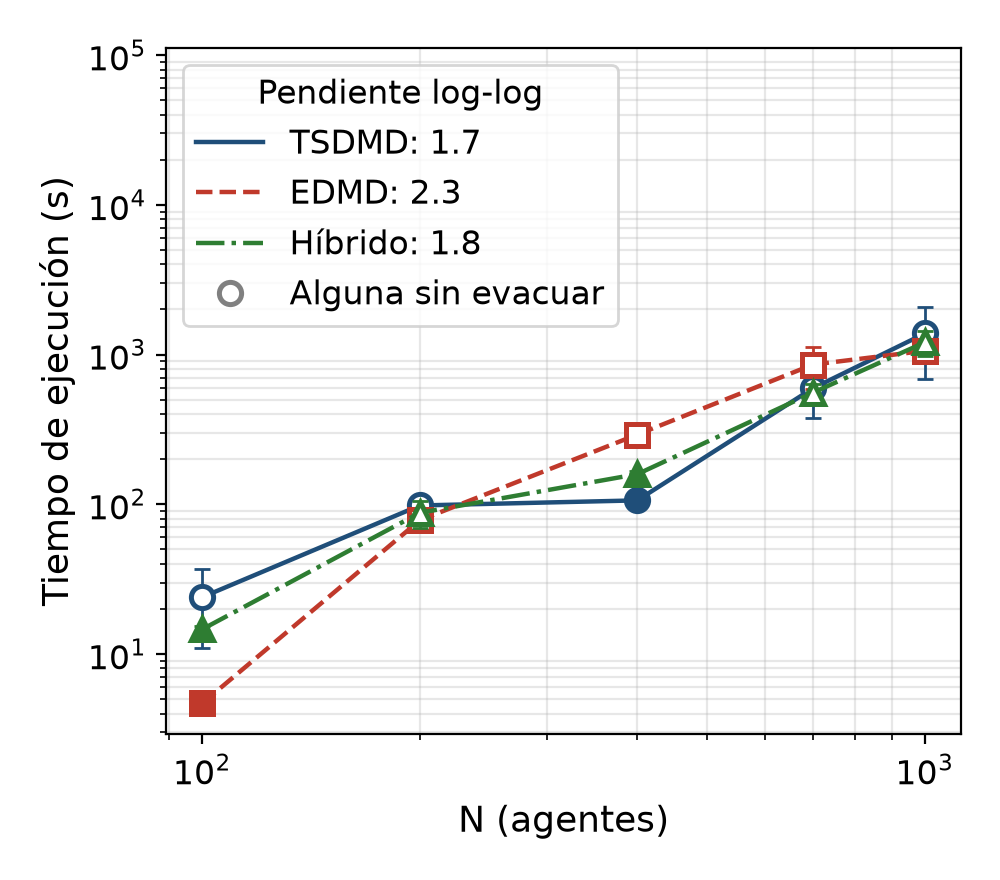
\includegraphics[width=\linewidth,height=0.84\textheight,keepaspectratio]{pres_scale_b.png}
    \end{column}
    \begin{column}{0.52\textwidth}
      \params{$N\in\{100,\,200,\,400,\,700,\,1000\}$, $L = 50\un{m}$,
      3 semillas por punto, $t_{max}\propto N$. Marcador hueco: alguna corrida llegó a $t_{max}$
      sin evacuar ($20$ de $45$).}

      \vspace{6pt}
      {\small Pendiente de la media observada: TSDMD $1.7$, EDMD $2.3$, híbrido $1.8$.
      \textbf{No son exponentes de costo.} Para $N\ge700$ los esquemas no se separan dentro
      del error con $3$ realizaciones por punto.}
    \end{column}
  \end{columns}
\end{frame}
